\documentclass[12pt]{standalone}
\usepackage{tikz, pgfmath}
\usetikzlibrary{calc, decorations.pathreplacing}


\begin{document}
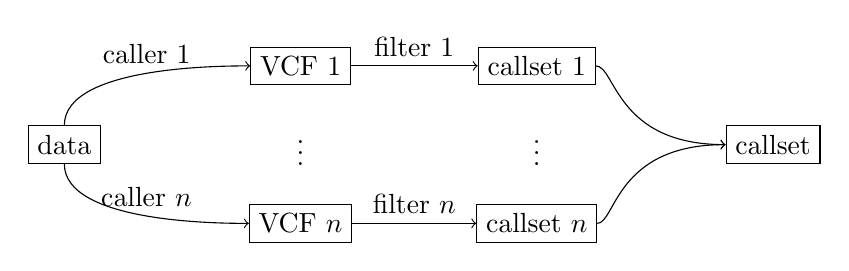
\begin{tikzpicture}[]
\node[draw] (data) at (0,0) {data};
\node[draw] (VCF1) at (3,1) {VCF \(1\)};
\node[draw] (callset1) at (6,1) {callset \(1\)};
\node (VCFi) at (3,0) {\(\vdots\)};
\node (callseti) at (6,0) {\(\vdots\)};
\node[draw] (VCFn) at (3,-1) {VCF \(n\)};
\node[draw] (callsetn) at (6,-1) {callset \(n\)};
\node[draw] (callset) at (9,0) {callset};

\draw[->] (data) .. controls +(up:1cm) and +(left:1cm).. node[midway, above] {caller \(1\)} (VCF1);
\draw[->] (data) .. controls +(down:1cm) and +(left:1cm).. node[midway, above] {caller \(n\)} (VCFn);

\draw[->] (VCF1) -- node[above] {filter \(1\)} (callset1);
\draw[->] (VCFn) -- node[above] {filter \(n\)} (callsetn);

\draw[->] (callset1) .. controls +(right:1cm) and +(left:2cm).. (callset);
\draw[->] (callsetn) .. controls +(right:1cm) and +(left:2cm).. (callset);
\end{tikzpicture}
\end{document}
